\documentclass[
%paper=5.5in:8.5in,
a5paper,
BCOR=7mm,
twoside,
DIV=calc,
11pt,
usegeometry,
chapterprefix,
headings=big]{scrbook} % Document font size and paper size

\usepackage{graphicx}
\usepackage{verse}
\usepackage{xcolor}
\usepackage{fontspec}
\usepackage[T1]{fontenc} % International character encodings
\usepackage{makeidx}
\usepackage{lettrine}
\usepackage{scrlayer-scrpage}
\usepackage{pifont}
\usepackage{enumitem}
\usepackage{caption}
\usepackage[maxlevel=3,autostyle]{csquotes}
\usepackage[export]{adjustbox}
\usepackage{polyglossia}
\usepackage{afterpage}
\usepackage{microtype}
\usepackage{tocbasic}
\usepackage[pass]{geometry}
\usepackage{setspace}
\usepackage{subfiles}
\usepackage{rotating}
\usepackage[all,defaultlines=2]{nowidow}
\usepackage{setspaceenhanced}
\usepackage{ebgaramond} 
\usepackage{floatpag}
\usepackage{pdfpages}

\MakeAutoQuote{»}{«}
\catcode`\—=13
%\protected\def—{\allowbreak\textemdash\allowbreak}
\protected\def—{\textemdash}
\newcommand\longdash{\mbox{---\,}\ignorespaces{}}

\floatpagestyle{empty}
\rotfloatpagestyle{empty}

\setmainfont{EB Garamond}
\setdefaultlanguage[variant=uk]{english}
\newcommand{\HUGE}{\fontsize{50}{60}\selectfont}
\newcommand{\moderatelyhuge}{\fontsize{50}{60}\selectfont}
\newcommand{\reasonablyhuge}{\fontsize{30}{40}\selectfont}
\newfontfamily\chapterfont{IMFeENsc28P.ttf}
\newfontfamily\chapterfontlower{IMFeENsc28P.ttf}



\addtokomafont{disposition}{\normalfont}

\renewcommand*{\partformat}{\partname~\thepart} %renew so it doesn't have the trailing period
\renewcommand*{\chapterformat}{\chaptername~\thechapter}
\newcommand*\hideentrynumber[1]{}
\makeatletter
\NewDocumentCommand\ArtPart{som}{%
  \cleardoubleevenpage
  \IfBooleanTF{#1}{% star version: no TOC entry or page header
  }{%
    \refstepcounter{part}%
    \IfValueTF{#2}{% optional argument: Use for TOC entry and page header
      \addparttocentry{\thepart.}{#2}%
      \partmark{#2}%
    }{}%
  }%
  \noindent\includegraphics[width=\textwidth]{#3}%
  \par\nobreak
  \@afterindentfalse% don't indent first paragraph after the heading
  \@afterheading% don't allow page break here etc.
  \thispagestyle{plain}
}
\NewDocumentCommand\ArtChapter{som}{%
  \cleardoubleoddpage
  \IfBooleanTF{#1}{% star version: no TOC entry or page header
  }{%
    \refstepcounter{chapter}%
    \IfValueTF{#2}{% optional argument: Use for TOC entry and page header
      \addchaptertocentry{\thechapter}{#2}%
      \chaptermark{#2}%
    }{}%
  }%
  \noindent\includegraphics[width=\textwidth]{#3}%
%  \par\nobreak
\vspace{0pt}
  \@afterindentfalse% don't indent first paragraph after the heading
  \@afterheading% don't allow page break here etc.
  \thispagestyle{plain}
}

\makeatother

\newcount\zzc
\makeatletter
\def\zz{%
\ifnum\prevgraf<\c@L@lines
\zzc\z@
\loop
\ifnum\zzc<\prevgraf
\advance\zzc\@ne
\afterassignment\zzda\count@\L@parshape\relax
\repeat
\parshape\L@parshape
\fi}
\def\zzda{\afterassignment\zzdb\dimen@}
\def\zzdb{\afterassignment\zzdef\dimen@}
\def\zzdef#1\relax{\edef\L@parshape{\the\numexpr\count@-1\relax\space #1}}
\makeatother

%\BeforeTOCHead[toc]{%
%  \KOMAoptions{parskip=false}% no parskip in ToC
%  \RedeclareSectionCommand[afterskip=1cm]{chapter}
%}
\BeforeTOCHead[tocline]{%
  \KOMAoptions{parskip=false}% no parskip in ToC
%  \RedeclareSectionCommand[afterskip=0pt]{figure}% no skip after ToC title
  \RedeclareSectionCommand[tocbeforeskip=1sp minus 1sp]{figure} %scootch entries together
}

\DeclareTOCStyleEntry[beforeskip=.1cm,dynnumwidth=true,linefill=\TOCLineLeaderFill]{chapter}{chapter}

\DeclareTOCStyleEntry[beforeskip=.3cm,dynnumwidth=true,entryformat=\Large\bfseries]{part}{part}
\DeclareTOCStyleEntry[beforeskip=.1cm,numwidth=-20pt,entrynumberformat=\hideentrynumber]{tocline}{figure}

%\DeclareTOCStyleEntry[beforeskip=.1cm,entryformat=\chapterfont,dynnumwidth=true,linefill=\TOCLineLeaderFill]{chapter}{chapter}
%
%\DeclareTOCStyleEntry[beforeskip=.3cm,dynnumwidth=true,entryformat=\Large\chapterfont\bfseries]{part}{part}
%\DeclareTOCStyleEntry[beforeskip=.1cm,numwidth=-20pt,entrynumberformat=\hideentrynumber]{tocline}{figure}

\DeclareTOCStyleEntry[beforeskip=.1cm]{tocline}{part}
\DeclareTOCStyleEntry[beforeskip=.1cm]{default}{subsection}



\headsep=10pt
\headheight=45pt
\footskip=30pt



%\defaultfontfeatures{Mapping=tex-text}
\defaultfontfeatures{Ligatures=TeX}



\automark{chapter}
\lehead{Treasure Island}
\rohead{Chapter \thechapter: \leftmark}
\flushbottom

\setlist[itemize]{noitemsep} 

\captionsetup[figure]{font=sc,labelformat=empty}

\graphicspath{ {./images/} }


\hyphenation{Bland-ly}


\begin{document}

\renewcommand*{\chaptermarkformat}{}
\renewcommand*{\chapterheadendvskip}{\vspace{0pt}}
\renewcommand*{\chapterheadstartvskip}{\vspace{0pt}}

\frontmatter
\pagestyle{empty}

% \recalctypearea
% \newgeometry{left=15mm,right=15mm,top=15mm,bottom=15mm}
 
 \includepdf[width=1.2\textwidth]{title.png}
 
 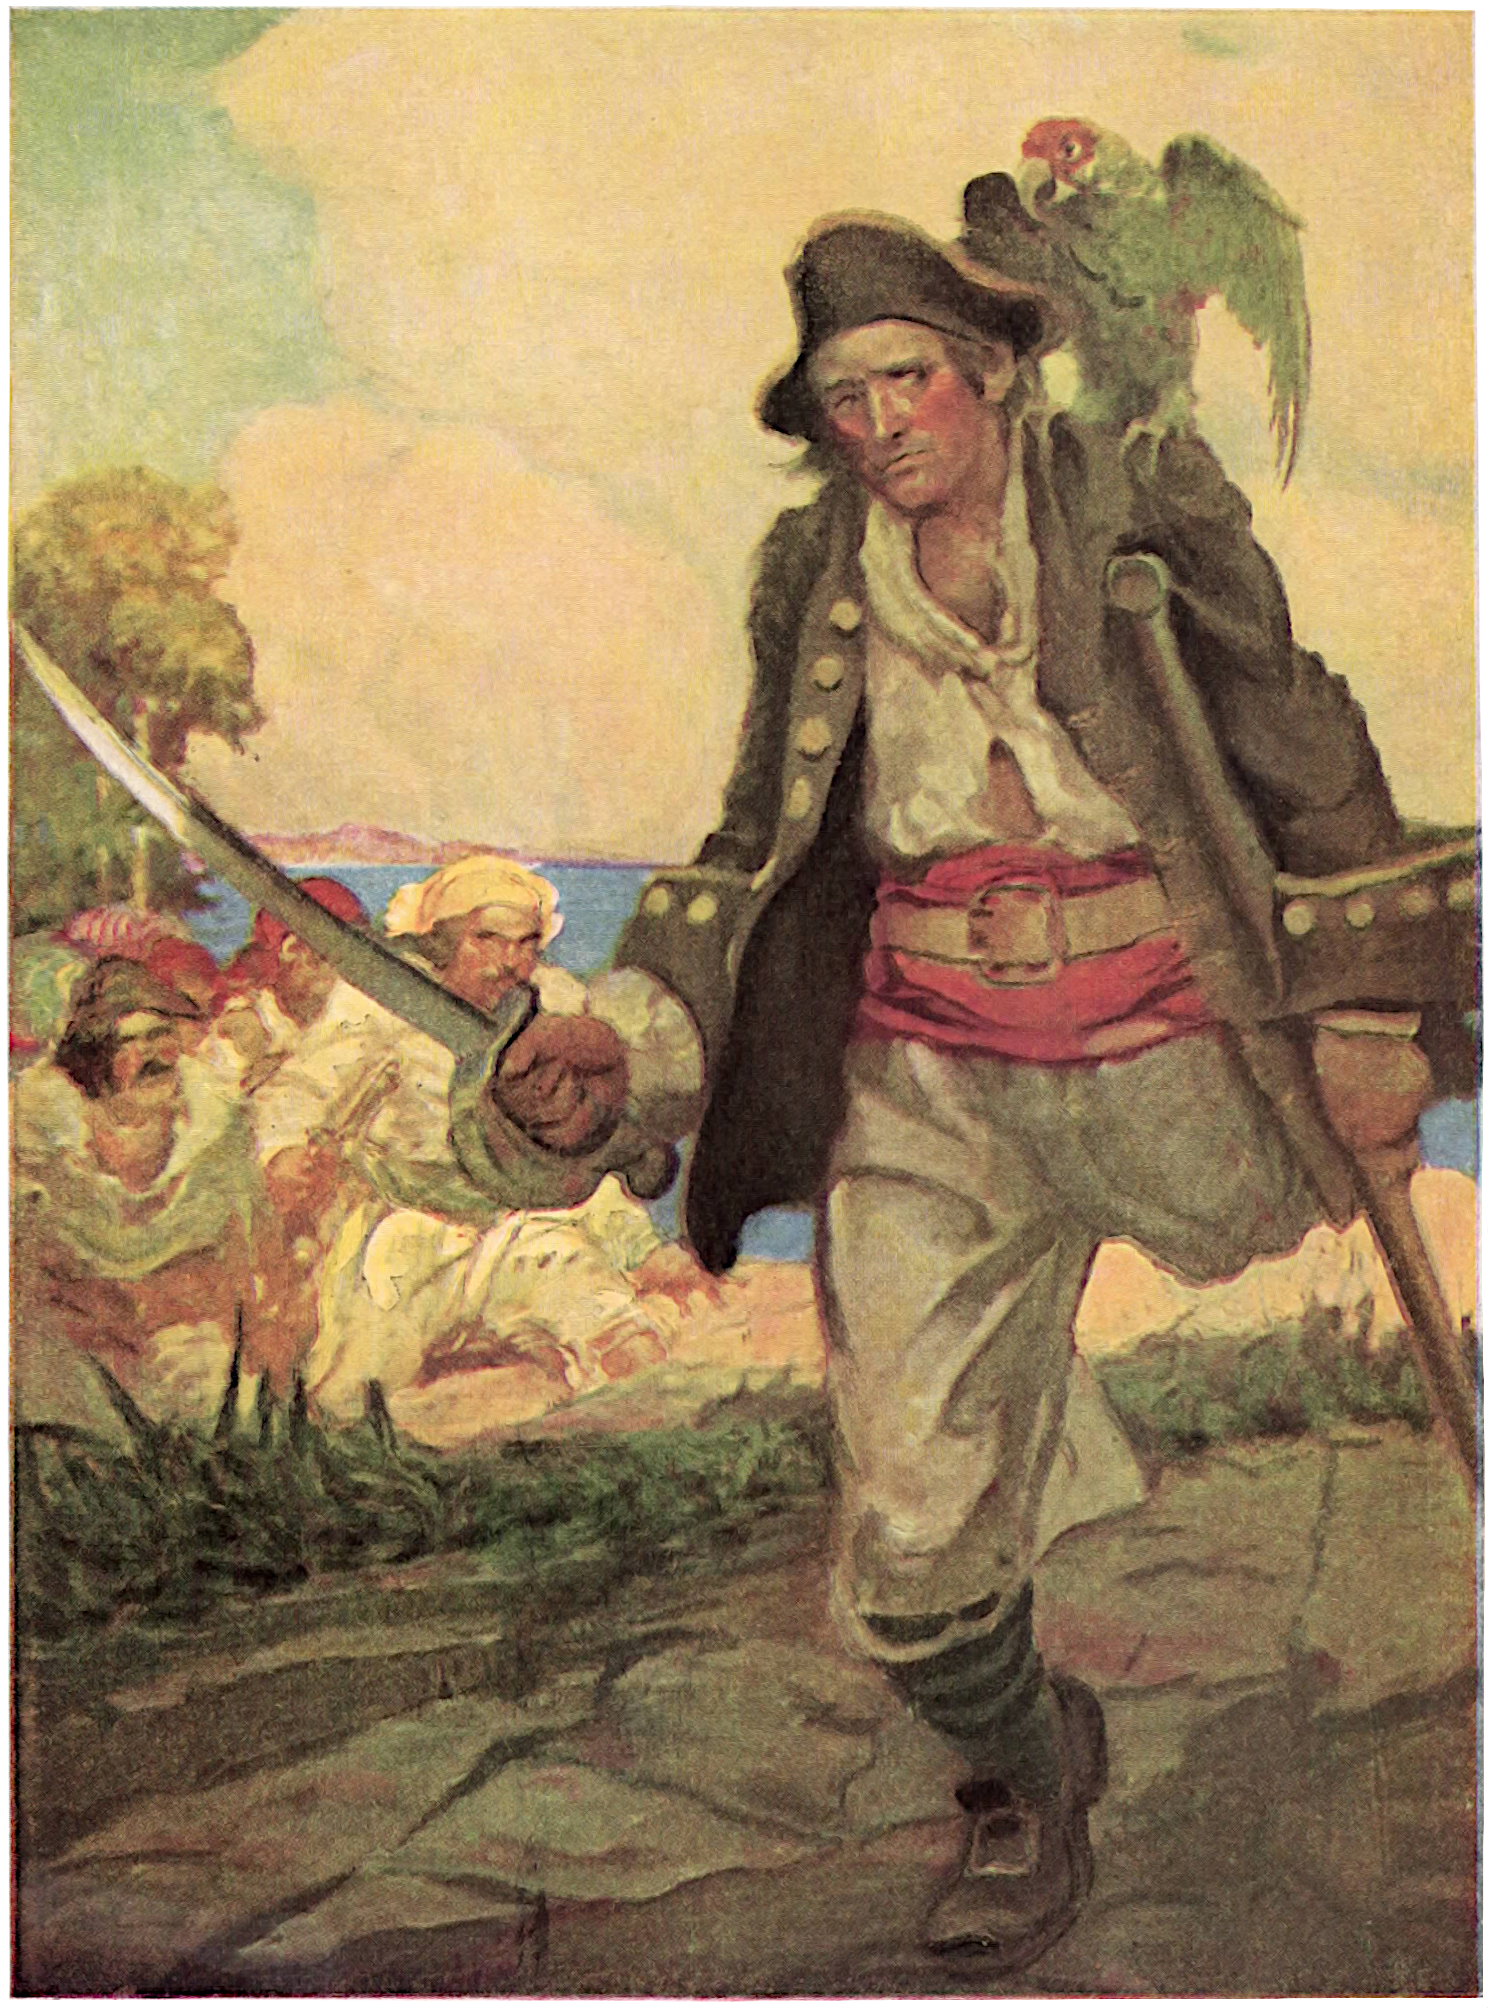
\includepdf[addtolist={1,figure,\textbf{Frontispiece},frontispiece},width=1.2\textwidth]{frontispiece.png}
 \includepdf[addtolist={1,figure,\textbf{Map},map},width=\textwidth]{timapcolor.png}
 
%	 
%	 \vfill
%	 \begin{figure}[p!]
%	\centering
%	\includegraphics[width=\hsize]{titlepage}
%	\end{figure}
%	\vfill
%	
%	
%	\KOMAoptions{headings=openany}
%	
%	
%	\vfill
%	 \begin{figure}[p!]
%	\centering
%	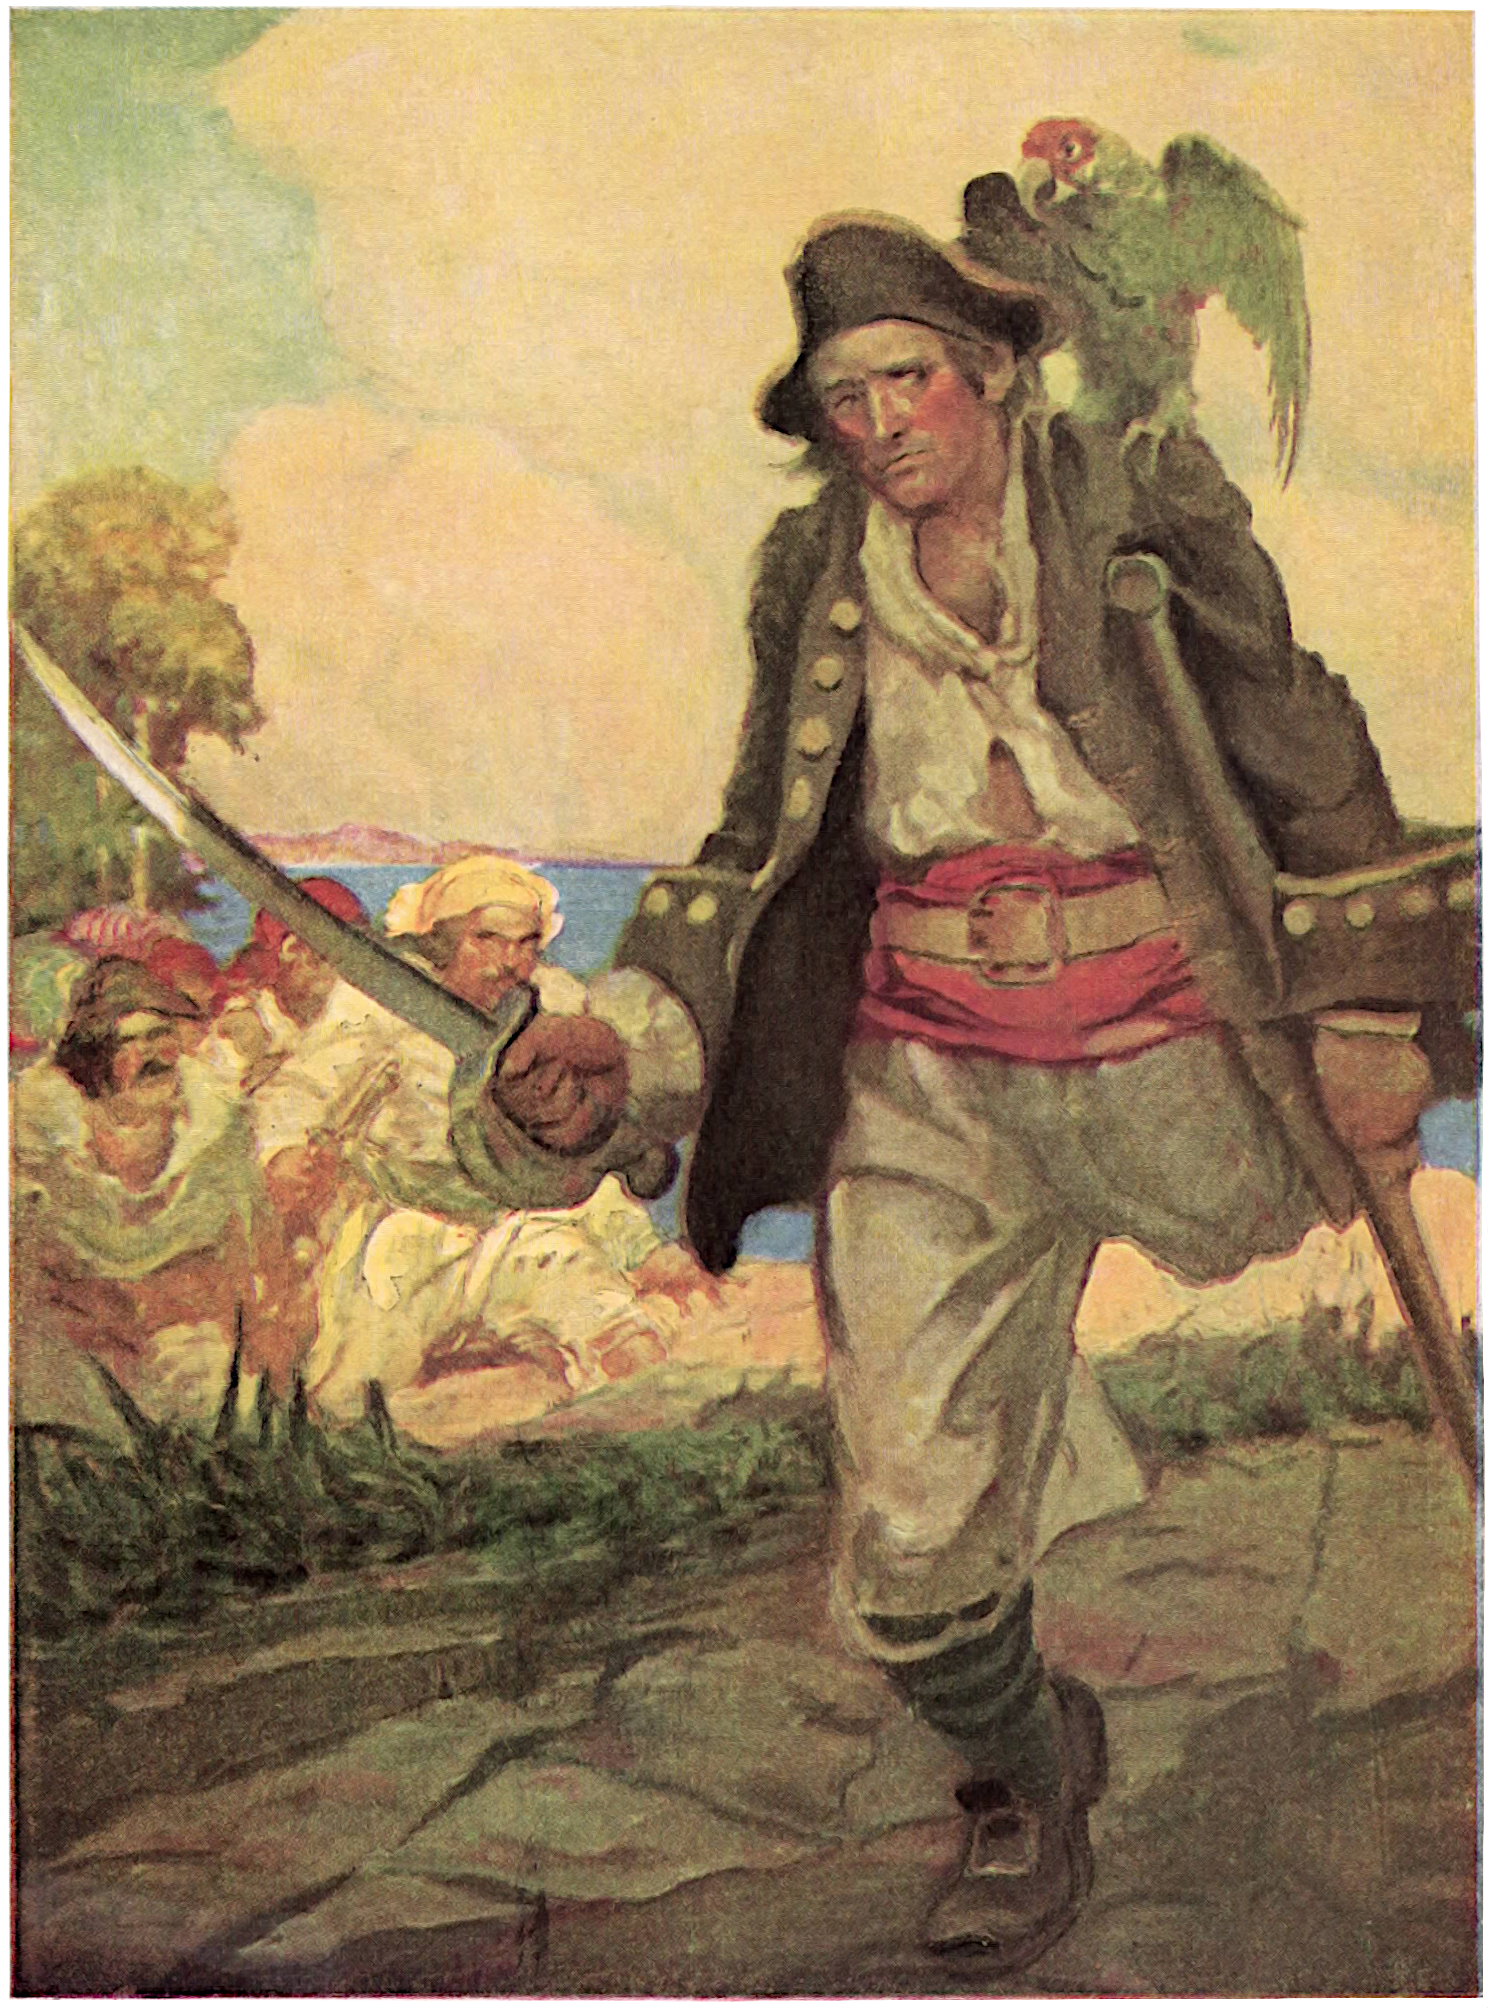
\includegraphics[width=\hsize]{frontispiece}
%	\caption[\textbf{Frontispiece}]{}
%	\end{figure}
%	\vfill
%	\thispagestyle{empty}
%	
%	
%	
%	~\vfill
%	 \begin{figure}[p!]
%	\centering
%	\includegraphics[width=\picsize]{timapcolor}
%	\caption[Map]{}
%	\end{figure}
%	~\vfill
%	\thispagestyle{empty}



\pagestyle{plain}

\renewcommand*\raggedchapter{\centering}
\KOMAoptions{headings=openleft}

%  \recalctypearea
%\restoregeometry

%\footskip=20pt
\renewcommand{\contentsname}{\includegraphics[width=\linewidth]{contents}}
\tableofcontents
%\clearpage




\renewcommand{\listfigurename}{\includegraphics[width=\linewidth]{listofillustrations}}
\listoffigures

%\clearpage



\footskip=30pt

\KOMAoptions{headings=openany}
\chapter*{Dedication}
~\\
~\\
\begin{center}\setstretch{1.8}\large
To\\
S.L.O.,\\ 
an American gentleman\\ 
in accordance with whose classic taste\\ 
the following narrative has been designed,\\ 
it is now, in return for numerous delightful hours,\\ 
and with the kindest wishes,\\
dedicated\\
 by his affectionate friend,\\
\begin{flushright}\scshape
the author.
\end{flushright}
\end{center}
\clearpage


\chapter*{To The Hesitating Purchaser}
\vfill
\settowidth{\versewidth}{Can please, as me they pleased of old,}
\begin{verse}[\versewidth]
\begin{altverse}
If sailor tales to sailor tunes,\\
Storm and adventure, heat and cold,\\
If schooners, islands, and maroons,\\
And buccaneers, and buried gold,\\
And all the old romance, retold\\
Exactly in the ancient way,\\
Can please, as me they pleased of old,\\
The wiser youngsters of today:\\!
---So be it, and fall on! If not,\\
If studious youth no longer crave,\\
His ancient appetites forgot,\\
Kingston, or Ballantyne the brave,\\
Or Cooper of the wood and wave:\\
So be it, also! And may I\\
And all my pirates share the grave\\
Where these and their creations lie!\\
\end{altverse}
\end{verse}
\vfill





{
\renewcommand{\cleardoublepage}{\newpage}
\mainmatter
}
\pagestyle{headings}
\renewcommand*{\chapterpagestyle}{plain}

\ArtPart[The Old Buccaneer]{part1head}


\KOMAoptions{headings=openright}
\include{chapters/01.tex}
\include{chapters/02.tex}
\include{chapters/03.tex}
\include{chapters/04.tex}
\include{chapters/05.tex}
\include{chapters/06.tex}

\KOMAoptions{headings=openleft}

\ArtPart[The Sea-Cook]{part2head}


\KOMAoptions{headings=openright}
\include{chapters/07.tex}
\include{chapters/08.tex}
\include{chapters/09.tex}
\include{chapters/10.tex}
\include{chapters/11.tex}
\include{chapters/12.tex}


\KOMAoptions{headings=openleft}

\ArtPart[My Shore Adventure]{part3head}

\KOMAoptions{headings=openright}
\include{chapters/13.tex}
\include{chapters/14.tex}
%!TeX root=../treasuretop.tex
\ArtChapter[The Man of the Island]{chap15head}

   \lettrine[lines=4,image=true]{chap15initF}{rom} the side of the hill, which was here steep and stony, a spout of gravel was dislodged and fell rattling and bounding through the trees. My eyes turned instinctively in that direction, and I saw a figure leap with great rapidity behind the trunk of a pine. What it was, whether bear or man or monkey, I could in no wise tell. It seemed dark and shaggy; more I knew not. But the terror of this new apparition brought me to a stand.

I was now, it seemed, cut off upon both sides; behind me the murderers, before me this lurking nondescript. And immediately I began to prefer the dangers that I knew to those I knew not. Silver himself appeared less terrible in contrast with this creature of the woods, and I turned on my heel, and looking sharply behind me over my shoulder, began to retrace my steps in the direction of the boats.

Instantly the figure reappeared, and making a wide circuit, began to head me off. I was tired, at any rate; but had I been as fresh as when I rose, I could see it was in vain for me to contend in speed with such an adversary. From trunk to trunk the creature flitted like a deer, running manlike on two legs, but unlike any man that I had ever seen, stooping almost double as it ran. Yet a man it was, I could no longer be in doubt about that.

I began to recall what I had heard of cannibals. I was within an ace of calling for help. But the mere fact that he was a man, however wild, had somewhat reassured me, and my fear of Silver began to revive in proportion. I stood still, therefore, and cast about for some method of escape; and as I was so thinking, the recollection of my pistol flashed into my mind. As soon as I remembered I was not defenceless, courage glowed again in my heart and I set my face resolutely for this man of the island and walked briskly towards him.

He was concealed by this time behind another tree trunk; but he must have been watching me closely, for as soon as I began to move in his direction he reappeared and took a step to meet me. Then he hesitated, drew back, came forward again, and at last, to my wonder and confusion, threw himself on his knees and held out his clasped hands in supplication.

At that I once more stopped.

\enquote{Who are you?} I asked.

\enquote{Ben Gunn,} he answered, and his voice sounded hoarse and awkward, like a rusty lock. \enquote{I’m poor Ben Gunn, I am; and I haven’t spoke with a Christian these three years.}

  \begin{figure}[p]
\centering
\includegraphics[width=\linewidth]{chap15poorbengunn}
\caption[\enquote{I’m poor Ben Gunn, I am}]{\enquote{I’m poor Ben Gunn, I am; marooned three years agone, and lived on goats since then.}}
\end{figure}

I could now see that he was a white man like myself and that his features were even pleasing. His skin, wherever it was exposed, was burnt by the sun; even his lips were black, and his fair eyes looked quite startling in so dark a face. Of all the beggar-men that I had seen or fancied, he was the chief for raggedness. He was clothed with tatters of old ship’s canvas and old sea-cloth, and this extraordinary patchwork was all held together by a system of the most various and incongruous fastenings, brass buttons, bits of stick, and loops of tarry gaskin. About his waist he wore an old brass-buckled leather belt, which was the one thing solid in his whole accoutrement.

\enquote{Three years!} I cried. \enquote{Were you shipwrecked?}

\enquote{Nay, mate,} said he; \enquote{marooned.}

I had heard the word, and I knew it stood for a horrible kind of punishment common enough among the buccaneers, in which the offender is put ashore with a little powder and shot and left behind on some desolate and distant island.

\enquote{Marooned three years agone,} he continued, \enquote{and lived on goats since then, and berries, and oysters. Wherever a man is, says I, a man can do for himself. But, mate, my heart is sore for Christian diet. You mightn’t happen to have a piece of cheese about you, now? No? Well, many’s the long night I’ve dreamed of cheese---toasted, mostly---and woke up again, and here I were.}

\enquote{If ever I can get aboard again,} said I, \enquote{you shall have cheese by the stone.}

All this time he had been feeling the stuff of my jacket, smoothing my hands, looking at my boots, and generally, in the intervals of his speech, showing a childish pleasure in the presence of a fellow creature. But at my last words he perked up into a kind of startled slyness.

\enquote{If ever you can get aboard again, says you?} he repeated. \enquote{Why, now, who’s to hinder you?}

\enquote{Not you, I know,} was my reply.

\enquote{And right you was,} he cried. \enquote{Now you---what do you call yourself, mate?}

\enquote{Jim,} I told him.

\enquote{Jim, Jim,} says he, quite pleased apparently. \enquote{Well, now, Jim, I’ve lived that rough as you’d be ashamed to hear of. Now, for instance, you wouldn’t think I had had a pious mother---to look at me?} he asked.

\enquote{Why, no, not in particular,} I answered.

\enquote{Ah, well,} said he, \enquote{but I had---remarkable pious. And I was a civil, pious boy, and could rattle off my catechism that fast, as you couldn’t tell one word from another. And here’s what it come to, Jim, and it begun with chuck-farthen on the blessed grave-stones! That’s what it begun with, but it went further’n that; and so my mother told me, and predicked the whole, she did, the pious woman! But it were Providence that put me here. I’ve thought it all out in this here lonely island, and I’m back on piety. You don’t catch me tasting rum so much, but just a thimbleful for luck, of course, the first chance I have. I’m bound I’ll be good, and I see the way to. And, Jim}---looking all round him and lowering his voice to a whisper---\enquote{I’m rich.}

I now felt sure that the poor fellow had gone crazy in his solitude, and I suppose I must have shown the feeling in my face, for he repeated the statement hotly: \enquote{Rich! Rich! I says. And I’ll tell you what: I’ll make a man of you, Jim. Ah, Jim, you’ll bless your stars, you will, you was the first that found me!}

And at this there came suddenly a lowering shadow over his face, and he tightened his grasp upon my hand and raised a forefinger threateningly before my eyes.

\enquote{Now, Jim, you tell me true: that ain’t Flint’s ship?} he asked.

At this I had a happy inspiration. I began to believe that I had found an ally, and I answered him at once.

\enquote{It’s not Flint’s ship, and Flint is dead; but I’ll tell you true, as you ask me---there are some of Flint’s hands aboard; worse luck for the rest of us.}

\enquote{Not a man---with one---leg?} he gasped.

\enquote{Silver?} I asked.

\enquote{Ah, Silver!} says he. \enquote{That were his name.}

\enquote{He’s the cook, and the ringleader too.}

He was still holding me by the wrist, and at that he give it quite a wring.

\enquote{If you was sent by Long John,} he said, \enquote{I’m as good as pork, and I know it. But where was you, do you suppose?}

I had made my mind up in a moment, and by way of answer told him the whole story of our voyage and the predicament in which we found ourselves. He heard me with the keenest interest, and when I had done he patted me on the head.

\enquote{You’re a good lad, Jim,} he said; \enquote{and you’re all in a clove hitch, ain’t you? Well, you just put your trust in Ben Gunn---Ben Gunn’s the man to do it. Would you think it likely, now, that your squire would prove a liberal-minded one in case of help---him being in a clove hitch, as you remark?}

I told him the squire was the most liberal of men.

\enquote{Aye, but you see,} returned Ben Gunn, \enquote{I didn’t mean giving me a gate to keep, and a suit of livery clothes, and such; that’s not my mark, Jim. What I mean is, would he be likely to come down to the toon of, say one thousand pounds out of money that’s as good as a man’s own already?}

\enquote{I am sure he would,} said I. \enquote{As it was, all hands were to share.}

\enquote{\textit{And} a passage home?} he added with a look of great shrewdness.

\enquote{Why,} I cried, \enquote{the squire’s a gentleman. And besides, if we got rid of the others, we should want you to help work the vessel home.}

\enquote{Ah,} said he, \enquote{so you would.} And he seemed very much relieved.

\enquote{Now, I’ll tell you what,} he went on. \enquote{So much I’ll tell you, and no more. I were in Flint’s ship when he buried the treasure; he and six along---six strong seamen. They was ashore nigh on a week, and us standing off and on in the old \textit{Walrus}. One fine day up went the signal, and here come Flint by himself in a little boat, and his head done up in a blue scarf. The sun was getting up, and mortal white he looked about the cutwater. But, there he was, you mind, and the six all dead---dead and buried. How he done it, not a man aboard us could make out. It was battle, murder, and sudden death, leastways---him against six. Billy Bones was the mate; Long John, he was quartermaster; and they asked him where the treasure was. \enquote{Ah,} says he, \enquote{you can go ashore, if you like, and stay,} he says; \enquote{but as for the ship, she’ll beat up for more, by thunder!} That’s what he said.}

\enquote{Well, I was in another ship three years back, and we sighted this island. \enquote{Boys,} said I, \enquote{here’s Flint’s treasure; let’s land and find it.} The cap’n was displeased at that, but my messmates were all of a mind and landed. Twelve days they looked for it, and every day they had the worse word for me, until one fine morning all hands went aboard. \enquote{As for you, Benjamin Gunn,} says they, \enquote{here’s a musket,} they says, \enquote{and a spade, and pick-axe. You can stay here and find Flint’s money for yourself,} they says.}

\enquote{Well, Jim, three years have I been here, and not a bite of Christian diet from that day to this. But now, you look here; look at me. Do I look like a man before the mast? No, says you. Nor I weren’t, neither, I says.}

And with that he winked and pinched me hard.

\enquote{Just you mention them words to your squire, Jim,} he went on. \enquote{Nor he weren’t, neither---that’s the words. Three years he were the man of this island, light and dark, fair and rain; and sometimes he would maybe think upon a prayer (says you), and sometimes he would maybe think of his old mother, so be as she’s alive (you’ll say); but the most part of Gunn’s time (this is what you’ll say)---the most part of his time was took up with another matter. And then you’ll give him a nip, like I do.}

And he pinched me again in the most confidential manner.

\enquote{Then,} he continued, \enquote{then you’ll up, and you’ll say this: Gunn is a good man (you’ll say), and he puts a precious sight more confidence---a precious sight, mind that---in a gen’leman born than in these gen’leman of fortune, having been one hisself.}

\enquote{Well,} I said, \enquote{I don’t understand one word that you’ve been saying. But that’s neither here nor there; for how am I to get on board?}

\enquote{Ah,} said he, \enquote{that’s the hitch, for sure. Well, there’s my boat, that I made with my two hands. I keep her under the white rock. If the worst come to the worst, we might try that after dark. Hi!} he broke out. \enquote{What’s that?}

For just then, although the sun had still an hour or two to run, all the echoes of the island awoke and bellowed to the thunder of a cannon.

\enquote{They have begun to fight!} I cried. \enquote{Follow me.}

And I began to run towards the anchorage, my terrors all forgotten, while close at my side the marooned man in his goatskins trotted easily and lightly.

\enquote{Left, left,} says he; \enquote{keep to your left hand, mate Jim! Under the trees with you! Theer’s where I killed my first goat. They don’t come down here now; they’re all mastheaded on them mountings for the fear of Benjamin Gunn. Ah! And there’s the cetemery}---cemetery, he must have meant. \enquote{You see the mounds? I come here and prayed, nows and thens, when I thought maybe a Sunday would be about doo. It weren’t quite a chapel, but it seemed more solemn like; and then, says you, Ben Gunn was short-handed---no chapling, nor so much as a Bible and a flag, you says.}

So he kept talking as I ran, neither expecting nor receiving any answer.

The cannon-shot was followed after a considerable interval by a volley of small arms.

Another pause, and then, not a quarter of a mile in front of me, I beheld the Union Jack flutter in the air above a wood.


\KOMAoptions{headings=openleft}
\ArtPart[The Stockade]{part4head}

\KOMAoptions{headings=openright}
\include{chapters/16.tex}
\include{chapters/17.tex}
\include{chapters/18.tex}
\include{chapters/19.tex}
\include{chapters/20.tex}
\include{chapters/21.tex}


\KOMAoptions{headings=openleft}
\ArtPart[My Sea Adventure]{part5head}

\KOMAoptions{headings=openright}
\include{chapters/22.tex}
\include{chapters/23.tex}
\include{chapters/24.tex}
\include{chapters/25.tex}
\include{chapters/26.tex}
\include{chapters/27.tex}

\KOMAoptions{headings=openleft}
\ArtPart[Captain Silver]{part6head}


\KOMAoptions{headings=openright}
\include{chapters/28.tex}
\include{chapters/29.tex}
\include{chapters/30.tex}
\include{chapters/31.tex}
\include{chapters/32.tex}
\include{chapters/33.tex}
\include{chapters/34.tex}



\clearpage

\KOMAoptions{headings=openleft}
\chapter*{}
\begin{figure}[t!]
\centering
\includegraphics[width=\linewidth]{colophon}
\end{figure}
\centering
\vspace{-0.3cm}
EB Garamond is Georg Mayr-Duffner's free and open source implementation of Claude Garamond’s famous humanist typefaces from the mid-sixteenth century. github.com/georgd/EB-Garamond

\rule{0.5\textwidth}{.4pt}

Title page, chapter titles, and part titles are set in IM Fell. Dr John Fell, Bishop of Oxford, purchased the original set of types from Holland circa 1670, for use by the University of Oxford. The Fell Types are digitally reproduced by Igino Marini. www.iginomarini.com


\rule{0.5\textwidth}{.4pt}

\textit{Treasure Island} was originally serialised in the magazine \textit{Young Folks} between 1881 and 1882, credited to the pseudononym »Captain George North«. In 1883, Cassell and Company published it in London (UK) as a standalone work, now credited to Robert Louis Stevenson (1850\textendash1894) under his own name. Illustrations by Louis Rhead (1857\textendash1926) are from the 1915 edition, published by Harper Brothers in New York City (USA). Grateful acknowledgement is made to the Internet Archive, which in 2007 digitised a copy of this edition belonging to the New York Public Library.

\rule{0.5\textwidth}{.4pt}


This typeset is dedicated to the public domain under a Creative Commons CC0 1.0 Universal deed: creativecommons.org/publicdomain/zero/1.0/\\

\rule{0.5\textwidth}{.4pt}

Typeset in \LaTeX{}. Last revised \today.
\enlargethispage{2\baselineskip}
\thispagestyle{empty}
\end{document}